\section{Results}

\begin{frame}{Teleportation}
\begin{figure} 
	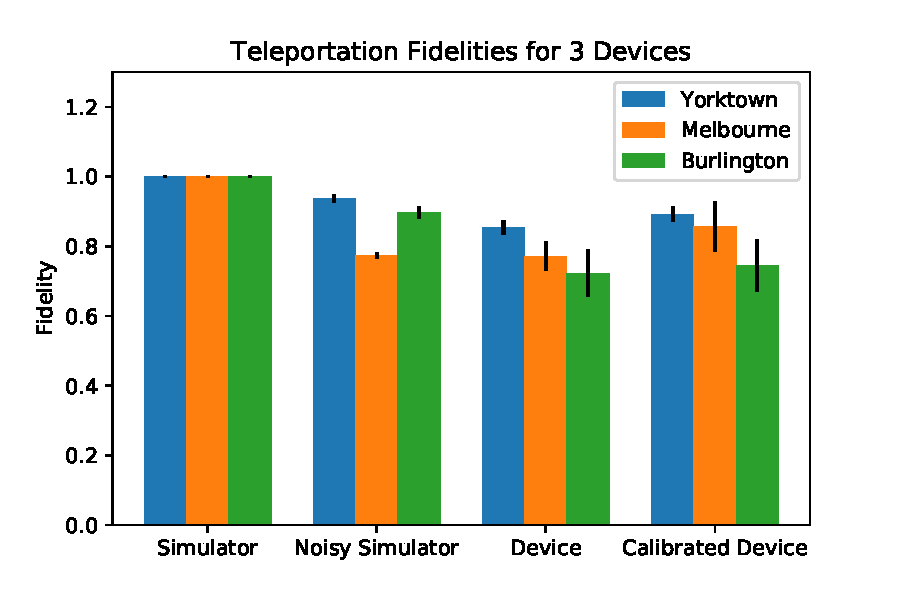
\includegraphics[width=1\textwidth]{images/results/teleport_histogram.pdf}
\end{figure}
\end{frame}

\begin{frame}{Entanglement Swapping}
\begin{figure} 
	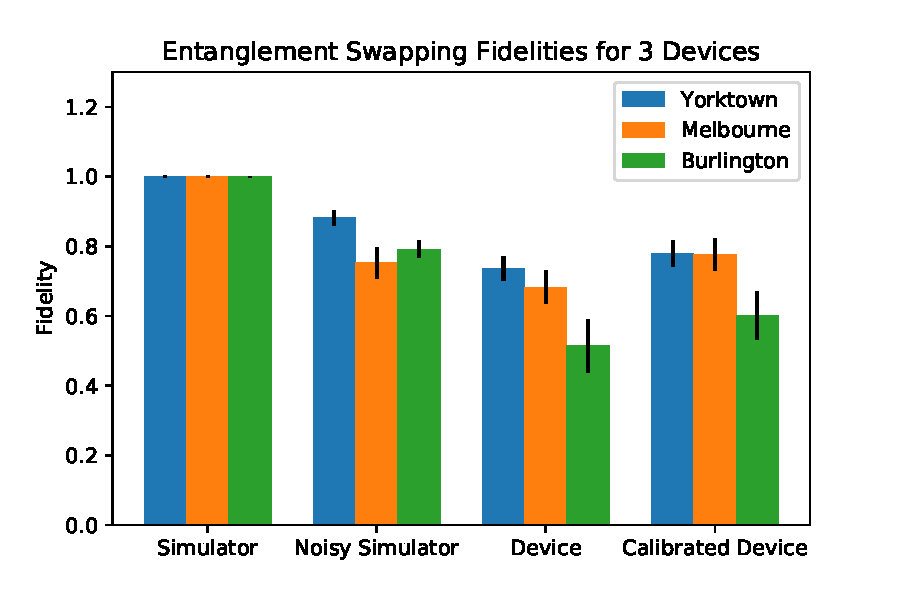
\includegraphics[width=1\textwidth]{images/results/swap_histogram.pdf}
\end{figure}
\end{frame}

\begin{frame}{Entanglement Purification}
\begin{figure}
	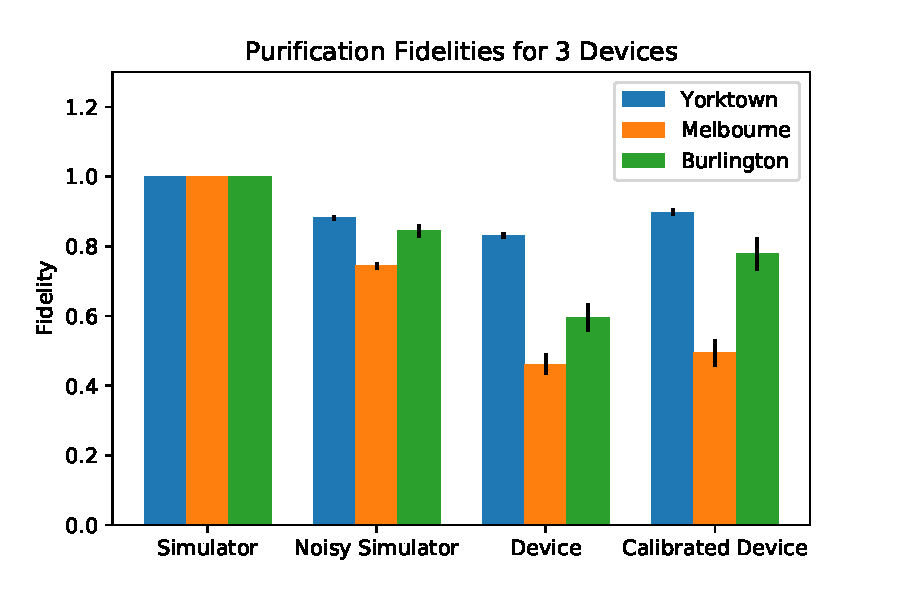
\includegraphics[width=1\textwidth]{images/results/purification_histogram.pdf}
\end{figure}
\end{frame}

\begin{frame}{Grover's Algorithm}
\begin{figure}
	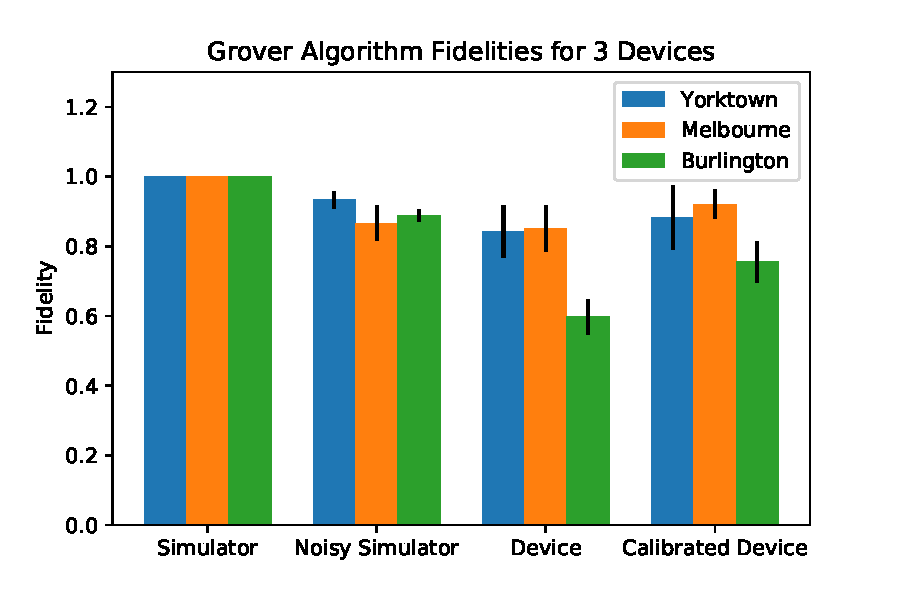
\includegraphics[width=1\textwidth]{images/results/grover_histogram.pdf}
\end{figure}
\end{frame}

\section{Conclusion/Future Outlook}
\begin{frame}{Conclusion/Future Outlook}
\begin{itemize}
	\item The circuit states were successfully reconstructed using one- and
	two-qubit state tomography.
	\item The optimal backend for implementation was Yorktown, since the advantages of greater inter-connectivity outweigh any disadvantage from slightly lower gate fidelities.
	\item Different types of circuits will favor implementation on qubits with very different physical properties.
	\item An
	interesting comparison to conduct might be the performance of different
	implementations with regards to a handful of well-known protocols.
\end{itemize}
\end{frame}
%%% Local Variables:
%%% mode: latex
%%% TeX-master: "presentation"
%%% End:
